\documentclass[ignorenonframetext,]{beamer}
\usefonttheme{structurebold}
\setbeamertemplate{caption}[numbered]
\setbeamertemplate{caption label separator}{:}
\setbeamercolor{caption name}{fg=normal text.fg}
\usepackage{amssymb,amsmath}
\usepackage{ifxetex,ifluatex}
\usepackage{fixltx2e} % provides \textsubscript
\usepackage{lmodern}
\ifxetex
  \usepackage{fontspec,xltxtra,xunicode}
  \defaultfontfeatures{Mapping=tex-text,Scale=MatchLowercase}
  \newcommand{\euro}{€}
\else
  \ifluatex
    \usepackage{fontspec}
    \defaultfontfeatures{Mapping=tex-text,Scale=MatchLowercase}
    \newcommand{\euro}{€}
  \else
    \usepackage[T1]{fontenc}
    \usepackage[utf8]{inputenc}
      \fi
\fi
% use upquote if available, for straight quotes in verbatim environments
\IfFileExists{upquote.sty}{\usepackage{upquote}}{}
% use microtype if available
\IfFileExists{microtype.sty}{\usepackage{microtype}}{}

% Comment these out if you don't want a slide with just the
% part/section/subsection/subsubsection title:
\AtBeginPart{
  \let\insertpartnumber\relax
  \let\partname\relax
  \frame{\partpage}
}
\AtBeginSection{
  \let\insertsectionnumber\relax
  \let\sectionname\relax
  \frame{\sectionpage}
}
\AtBeginSubsection{
  \let\insertsubsectionnumber\relax
  \let\subsectionname\relax
  \frame{\subsectionpage}
}

\setlength{\parindent}{0pt}
\setlength{\parskip}{6pt plus 2pt minus 1pt}
\setlength{\emergencystretch}{3em}  % prevent overfull lines
\setcounter{secnumdepth}{0}
%---- 
\institute{\faUniv 横浜国立大学大学院 環境情報学府 酒井研究室}
%----
\definecolor{Black1}{RGB}{50, 43, 38}
\definecolor{Orange1}{RGB}{244, 54, 21}
\definecolor{Beige1}{RGB}{236, 237, 227}
\definecolor{Navy1}{RGB}{16, 126, 137}
\definecolor{Grey1}{RGB}{164, 173, 185}
\definecolor{Yellow1}{RGB}{242, 163, 25}

\usepackage{zxjatype}
\setjamainfont{Hiragino Kaku Gothic Pro}
\setmainfont{Arial Black}
\usepackage{fontspec, fontawesome}
\usepackage{scrextend}
\changefontsizes{22pt}
\usepackage{nruby}

\setbeamercolor{background canvas}{bg = Beige1}
\setbeamertemplate{navigation symbols}{}
\setbeamertemplate{frametitle}[default][center]
\setbeamertemplate{itemize items}{\textcolor{Navy1}{\faCaretRight}}
\setbeamerfont{title}{size = \fontsize{46}{10}}
\setbeamercolor{title}{fg = Black1}
\setbeamercolor{author}{fg = Black1}
\setbeamercolor{normal text}{fg = Black1}
\setbeamerfont{date}{series = \itshape, size = \footnotesize}
\setbeamercolor{date}{fg = Grey1}
\setbeamerfont{frametitle}{size = \LARGE}
\setbeamercolor{frametitle}{fg = Navy1}
\renewcommand{\baselinestretch}{1.0}

% define font awesome
\providecommand\faGit{{\FA\symbol{"F1D3}}}
\providecommand\faGitSquare{{\FA\symbol{"F1D2}}}
\providecommand\faBomb{{\FA\symbol{"F1E2}}}
\providecommand\faTree{{\FA\symbol{"F1BB}}}
\providecommand\faUniv{{\FA\symbol{"F19C}}}

\title{生態学者が \textcolor{Orange1}{\faGit} を使うべき理由}
\author{瓜生真也}
\date{January 24, 2015 \newline 日本生態学会関東地区会公開シンポジウム}

\begin{document}
\frame{\titlepage}

\begin{frame}

\center{
  \huge{\textbf{\rotatebox{-20}{$\backslash$研究の話はなし\slash}}}
  \small{懇親会のときに}
}

\end{frame}

\begin{frame}

\center{
  \textbf{\Large{LTの内容}\\\Huge{研究の\textcolor{Orange1}{再現性}に関する話}}
}

\end{frame}

\begin{frame}{\faBeaker 再現性}

\begin{itemize}
\itemsep1pt\parskip0pt\parsep0pt
\item
  昔から科学につきまとう問題
\item
  論文の内容を第三者が再現できるか
\item
  \textbf{再現性の高い研究 $\fallingdotseq$ 良い研究}
\end{itemize}

\end{frame}

\begin{frame}

\center{
  \Huge{ところが...}
}

\end{frame}

\begin{frame}{\faWarningSign 研究中に陥る闇}

\center{
  \Large{論文原稿のファイル名を\\改訂の度に変更する}
  
  \scriptsize{\textit{
    \textcolor{Grey1}{
      \faFileAlt manuscript$\_$v0.1.tex\\
      \faFileAlt manuscript$\_$v1.0.tex\\
      \faFileAlt manuscript$\_$v2.2.tex}\\
    \textcolor{Orange1}{
      \faFileAlt \textbf{manuscript$\_$submit.tex}}
  }}
  
  各種混乱の元...
}

\end{frame}

\begin{frame}{\faWarningSign 研究中に陥る闇}

\center{
  \Large{自分で書いた\\解析用のコードの意味が\\わからない\\}
  
  \scriptsize{昔はできたのに...}
}

\end{frame}

\begin{frame}{闇は深い}

\begin{itemize}
\itemsep1pt\parskip0pt\parsep0pt
\item
  モデルごとにファイルを用意\ldots{}\newline 増殖したファイルが散乱
\item
  意味不明なファイル名 (ex. あ.R, temp.txt)
\item
  再現性の低いエクセルでの作業
\item
  削除して良いかわからないファイル
\end{itemize}

\end{frame}

\begin{frame}

\center{
  \fontsize{240}{10}{\rotatebox{-30}{\faThumbsDown}}
}

\end{frame}

\begin{frame}

\center{
  \Huge{\textbf{一筋の\textcolor{Yellow1}{光明}}}
}

\end{frame}

\begin{frame}

\center{
  \huge{ぎっと}
  
  \textcolor{Orange1}{\fontsize{200}{10}{\faGitSquare}}
}

\end{frame}

\begin{frame}{\textcolor{Orange1}{\faGit}とはなにか}

\begin{itemize}
\itemsep1pt\parskip0pt\parsep0pt
\item
  \textbf{分散型}バージョン管理システム

  \begin{itemize}
  \itemsep1pt\parskip0pt\parsep0pt
  \item
    コンピュータのソースコード開発・管理のために作られた
  \item
    リポジトリによるローカル環境でのファイル管理

    \begin{itemize}
    \itemsep1pt\parskip0pt\parsep0pt
    \item
      複数人での作業にも効果的
    \end{itemize}
  \end{itemize}
\end{itemize}

\end{frame}

\begin{frame}{作業内容の履歴}

\center{
  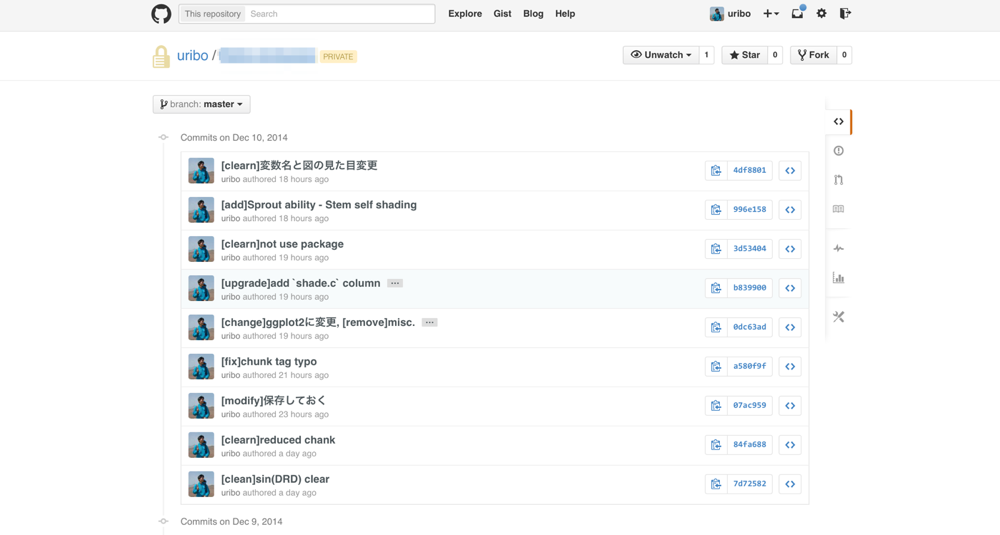
\includegraphics[width = 11cm]{images/git_commit_history.pdf}
}

\end{frame}

\begin{frame}{差分表示}

\center{
  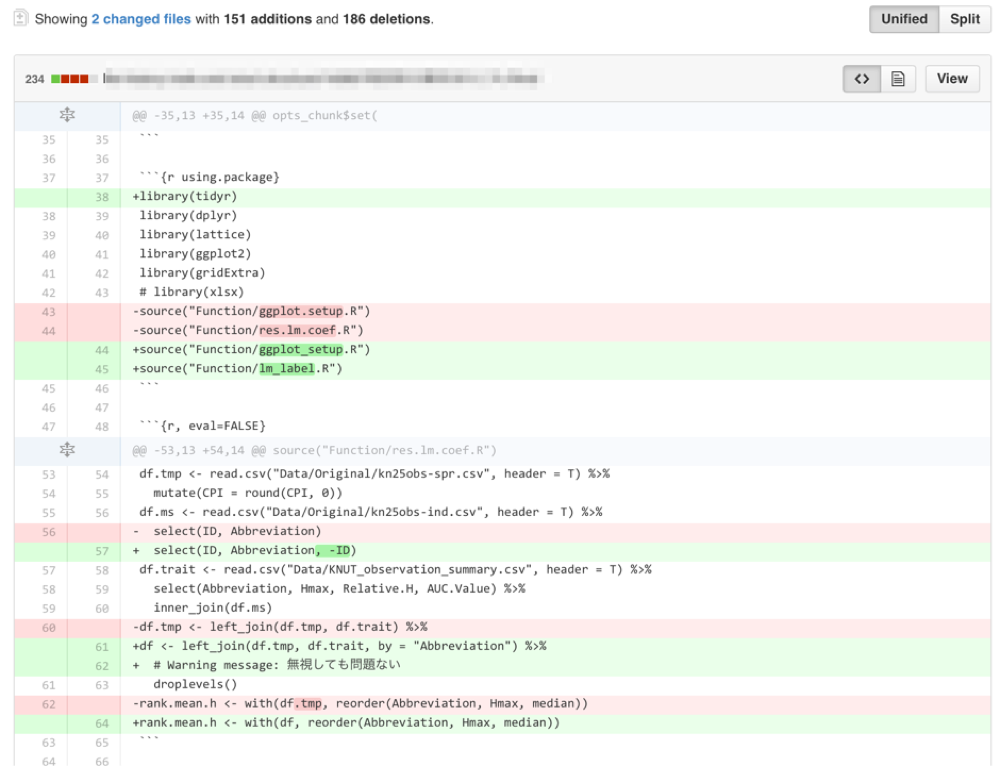
\includegraphics[width =11cm]{images/git_diff.pdf}
}

\end{frame}

\begin{frame}{差分表示(画像ファイル)}

\tiny{https://github.com/cameronmcefee/Image-Diff-View-Modes/}

\center{
  \includegraphics[width =11cm]{images/github_image_diff.pdf}
}

\end{frame}

\begin{frame}{\Large{どんなにかすれたインクでも、\\最高の記憶力に勝る}}

長い時間をかけて研究は完成する

\faHandLeft \textbf{いつ、誰が、なにをしたのか}を記録しておくことが大事

\end{frame}

\begin{frame}

\center{
  \huge{GitHub}
  \fontsize{200}{10}{\faGithub}
}

\end{frame}

\begin{frame}{\faGithub GitHubとはなにか}

\begin{itemize}
\itemsep1pt\parskip0pt\parsep0pt
\item
  \textcolor{Orange1}{\faGit}リポジトリのホスティングサイト
\item
  公開されたリポジトリの開発に参加できる
\item
  学生、研究組織であれば無料で非公開リポジトリを作成可能
\end{itemize}

\end{frame}

\begin{frame}{\faGithub GitHub活用事例: \newline Rパッケージ}

開発、配布は \newline CRAN \faArrowRight \textbf{GitHubが主流に}

\tiny{例) taxizeパッケージ (https://github.com/ropensci/taxize)}

\texttt{devtools::install\_github("taxize", "ropensci")}

\end{frame}

\begin{frame}{\faGithub GitHub活用事例: \newline BADD}

\footnotesize{https://github.com/dfalster/baad}

\begin{itemize}
\itemsep1pt\parskip0pt\parsep0pt
\item
  \scriptsize{\textit{a Biomass And Allometry Database for woody plants}}
\item
  \scriptsize{データおよび使用したRコードを公開}
\item
  \scriptsize{Ecologyに投稿中とのこと}
\end{itemize}

\end{frame}

\begin{frame}{\faGithub GitHub活用事例:
\newline \normalsize{第35回関東地区生態学関係修士論文発表会}}

\tiny{https://github.com/esj-kantomaster/esj-kantomaster.github.io}

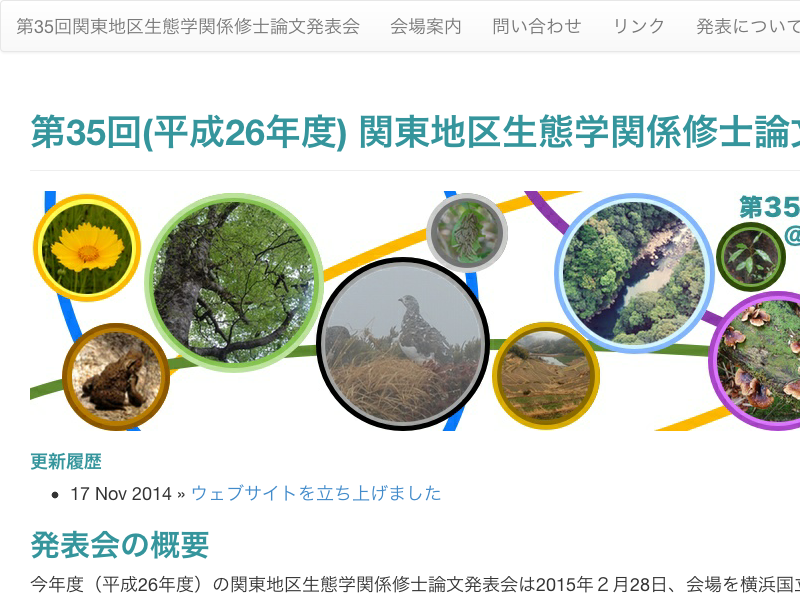
\includegraphics[width = 11cm]{images/webshot_esj_master_kanto.pdf}

\end{frame}

\begin{frame}{\large{Reproducible Research \newline に対する機運}}

\begin{columns}[T]
  \begin{column}[T]{4cm}
    \tiny{\faFile Ram, K. (2013). \textcolor{Orange1}{\textbf{Git can facilitate greater reproducibility and increased transparency in science}}. \textit{Source Code for Biology and Medicine}}\\
    \tiny{\faFile Peng, R. D. (2011). \textit{Science}}\\
    \tiny{\faFile Loman, N., \& Watson, M. (2013). \textit{Nature Biotechnology}}
  \end{column}
  \begin{column}[T]{6cm}
    \tiny{http://www.nature.com/news/toolbox}\\
    \includegraphics[width = 6cm]{images/reproducible_research.pdf}\\
  \end{column}
\end{columns}

\end{frame}

\begin{frame}{\faBullhorn Try \textcolor{Orange1}{\faGit}}

\center{
  \huge{\textbf{\textcolor{Orange1}{\faUser 自分のため、\\\faGroup 仲間のため、\\\faGlobe 誰かのため}}}
}

\end{frame}

\end{document}
